\newpage
\section{实验练习}
\begin{exercise}\label{exer:5.1}
样品池中加入一滴甲苯,盖盖,密封,在220--280 nm范围内测试气相吸收光谱。保持扫描
速率,改变狭缝宽度,如0.1、0.5、1和5 nm。请解释不同的狭缝宽度导致的不同光谱
解析率。
\end{exercise}
\begin{exercise}\label{exer:5.2}
记录正辛烷的吸收光谱;在220--280 nm记录体积比为0.02\%的甲苯正辛烷的吸收光谱。
如果使用双光束光谱仪,正辛烷可以放置于参比池中。对比练习\ref{exer:5.1}结果,
解释你观察到的现象。按照相同方式改变狭缝宽度,观察解析率的变化。
\end{exercise}
\begin{exercise}\label{exer:5.3}
在200--400 nm范围内,记录(a)1-辛烯(b)1,3-丁二烯(c)非共轭二烯(1,4-戊二烯)的
吸收光谱。共轭体系有什么特点?光谱给出每个化合物分子轨道能量什么信息?
\end{exercise}
\begin{exercise}\label{exer:5.4}
记录多核芳香族化合物(如蒽)和醌类(如苯醌)的吸收光谱。不同的结构带来什么不同
的光谱?
\end{exercise}
\begin{exercise}\label{exer:5.5}
参照练习\ref{exer:5.2},为甲苯选择合适的吸收波长,相对于0.02\%的溶液,制备一
系列浓度的甲苯正辛烷溶液(例如,体积比为0.1\%、0.05\%和0.01\%),使用正辛烷做
参比,测量溶液的吸光度。
\end{exercise}
\begin{exercise}\label{exer:5.6}
练习\ref{exer:5.5}获得的吸收数据,绘制吸光度$A$相对于浓度$c$的吸收曲线,并表明
分析范围。
\end{exercise}
\begin{exercise}\label{exer:5.7}
将适量奎宁溶于水制备奎宁标准溶液,记录溶液在200--500 nm之间的吸收光谱。测试几个
商业品牌奎宁水溶液的吸收光谱(鼓泡后)。哪个品牌的奎宁含量高?
\end{exercise}
\begin{exercise}\label{exer:5.8}
将250 g醋酸铵溶解在150 mL去离子水中,然后添加700 mL冰醋酸,制备醋酸铵缓冲溶液。
将1,10-菲啰啉一水合物100 mg溶于100 mL去离子水中,加入HCl。1 mL这种溶液与100
$\mu$g亚铁离子反应。在1 g/L的硫酸亚铁储液取0、100、200、300和400 $\mu$g的
\ce{Fe^{2+}}于100 mL的容量瓶中,加2 mL盐酸,加10 mL醋酸铵缓冲溶液,加4 mL配置
好的1,10-菲啰啉溶液,去离子水稀释至刻度线。混合均匀,静止15分钟以显色。510 nm
测量吸光度,绘制吸光度-浓度曲线。
\end{exercise}
\begin{exercise}\label{exer:5.9}
准确称量20 mg对乙酰氨基酚,溶于2 mL甲醇,去离子水定容于100 mL容量瓶中,制成储液
。取3 mL储液,定容于100 mL。以相同的方法,制备对乙酰氨基酚测试样品。在1 cm的
石英样品池、244 nm下测量样品的吸光度(减去溶剂空白)。并计算
\[
\text{试样量}=\text{标准样重量(mg)}\times\frac{\text{试样吸光度}}{\text{
标准样吸光度}}
\]
\[
\text{纯度}=100\times\frac{\text{测试样重量计算值}}{\text{测试样重量精确值}}
\]
\end{exercise}
\begin{exercise}\label{exer:5.10}
鼻喷雾剂过去曾含有L-去氧肾上腺素(PEH)和马来酸氯苯那敏(PAM)。
(当前的配方可能有所不同)准备以下溶液:(a)1升0.10 M HCl;(b)1 L PEH储备溶液,
其中包含200($\pm$10) mg的PEH在0.010 M HCl中,并记录实际浓度;(c)1 L PAM储备
溶液,其中含有80($\pm$5) mg PAM在0.010 M HCl中,并记录浓度。记录每种储备溶液的
UV光谱,范围为230至300 nm。为PEH选择最佳波长,为PAM选择最佳波长。使用PEH储备
溶液和10 mL容量瓶,通过稀释储备溶液组成6个标准溶液,其吸收范围从0到1。每种溶液
应为0.010 M的HCl。那你的空白是什么?记录每种标准溶液的浓度。对您的PAM库存溶液
执行相同的操作。在您选择的两个波长下,记录所有溶液(每种化合物的空白标准液
和6个标准液)的吸光度测量值。使用绘图程序(或坐标纸)获得两种波长下PEH和PAM的
Beer定律图。它们是线性的吗?使用最小二乘法程序,获得比尔定律图的斜率,截距和
相关系数。接下来,准备同时包含PEH和PAM的三种溶液。记录两个波长的吸光度。吸光度
值可加吗?如果您使用的是鼻喷雾剂,在分析天平上称量0.5 g,使用0.010 M HCl将其
稀释200份,每1份稀释一次。最简单的方法是将喷雾喷到天平上去皮的10 mL烧杯中。将
样品倒入100 mL容量瓶中,然后用0.010 M HCl冲洗烧杯多次,将洗涤液添加到容量瓶中,
使其达到刻度。这应该一式三份。记录三个样品在两个波长下的吸光度。建立并求解
联立方程。计算稀释样品中PEH和PAM的平均百分比。确定标准偏差。将结果报告给正确
数量的有效数字。(实验由纽约州斯克内克塔迪联合大学化学系T.C. Werner教授提供。)
\end{exercise}
\newpage
\begin{problemset}
\item 分子在紫外下激发有哪些类型?为什么?
\item 标明并解释下列分子紫外吸收类型:(a)庚烷(b)苯(c)1,3-丁二烯(d)水(e)1-庚烯
    (f)1-氯己烷(g)乙醇(h)氨水(i)正丁胺
\item 画出双光束光谱仪结构图,并简述主要部件功能
\item 列出UV/VIS主要光源
\item 640 nm波长的辐射通过简单的光栅单色仪,以20$^\circ$角分散,该光栅以相同
    角度还能分散什么波长辐射(最低200 nm)?
\item 解释PMT操作原理
\item 紫外吸收光谱定性分析有哪些局限性?
\item (a)依据下表数据,绘制氯苯标准吸收曲线(b)依据所绘制曲线,透过率分别为90\%
    、85\%和80\%的三种样品,氯苯浓度各是多少?

    \begin{center}
    \begin{tabular}{lc}
        \hline
        浓度(ppm) & 吸光度 \\
        \hline
        1.2 & 0.24 \\
        2.5 & 0.50 \\
        3.7 & 0.71 \\
        5.1 & 0.97 \\
        7.2 & 1.38 \\
        9.8 & 1.82 \\
        \hline
    \end{tabular}
    \end{center}
\item 现有如下氯苯吸收数据,使用上例标准吸收曲线,回答(a)样品A到D的浓度是多少?
    (b)样品E测试有什么问题?怎么分析所得数据?

    \begin{center}
    \begin{tabular}{lc}
        \hline
        样品编号  &  吸光度 \\
        \hline
        A & 0.400 \\
        B & 0.685 \\
        C & 0.120 \\
        D & 0.160 \\
        E & 3.000 \\
        \hline
    \end{tabular}
    \end{center}
\item 下述分子中,在紫外区域有吸收的是?(a)\ce{N2};(b)\ce{O2};(c)\ce{O3};(d)\ce{
    CO2};(e)\ce{CH4};(f)\ce{C2H4};(g)\ce{I2};(h)\ce{Cl2};(i)环己烷;(j)\ce{C3H6}
\item 为什么酚酞在酸和碱中变色?
\item 为什么紫外吸收光谱是宽带?
\item 什么导致光谱蓝移和红移?
\item 为什么氘灯发射连续非线性光谱?
\item p-n型二极管如何工作的?
\item 描述二极管阵列
\item 描述紫外过程的分子荧光和磷光
\item 荧光和激发光强度$I_0$是什么关系?
\item 解释分析物浓度增大,荧光强度逆转,怎么修正误差?
\item 画出测量紫外荧光强度的设备图
\item (a)紫外荧光有哪些干扰?(b)为什么磷光不像荧光那样在分析测量中广泛使用?
\item 从图\ref{fig:5.59}奎宁和蒽的发射光谱中,选择一个波长,可以确定奎宁和蒽
    混合物中奎宁的含量。蒽的相同。可以使用发射光谱来区分两种化合物吗?为什么?
\item 计算下列物质最大吸收波长
    \begin{figure}[h]
        \subcaptionbox{}{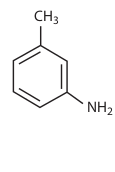
\includegraphics{2021-01-26_17-09.png}}
        \subcaptionbox{}{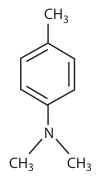
\includegraphics{2021-01-26_17-09_1.png}}
        \subcaptionbox{}{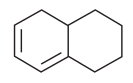
\includegraphics{2021-01-26_17-14.png}}
        \subcaptionbox{}{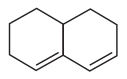
\includegraphics{2021-01-26_17-14_1.png}}
        \subcaptionbox{}{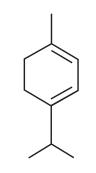
\includegraphics{2021-01-26_17-14_2.png}}
        \subcaptionbox{}{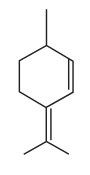
\includegraphics{2021-01-26_17-14_3.png}}
        \subcaptionbox{}{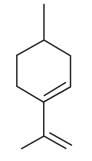
\includegraphics{2021-01-26_17-14_4.png}}
        \subcaptionbox{}{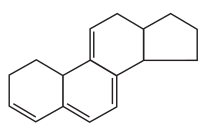
\includegraphics{2021-01-26_17-15.png}}
        \subcaptionbox{}{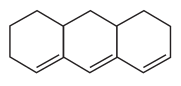
\includegraphics{2021-01-26_17-15_1.png}}
        \subcaptionbox{}{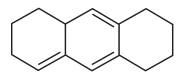
\includegraphics{2021-01-26_17-15_2.png}}
        \subcaptionbox{}{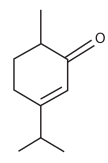
\includegraphics{2021-01-26_17-15_3.png}}
        \subcaptionbox{}{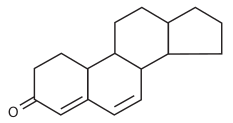
\includegraphics{2021-01-26_17-15_4.png}}
        \subcaptionbox{}{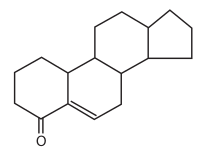
\includegraphics{2021-01-26_17-16.png}}
        \subcaptionbox{}{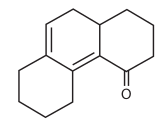
\includegraphics{2021-01-26_17-16_1.png}}
        \subcaptionbox{}{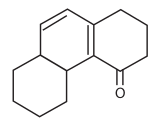
\includegraphics{2021-01-26_17-16_2.png}}
        \subcaptionbox{}{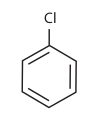
\includegraphics{2021-01-26_17-16_3.png}}
        \subcaptionbox{}{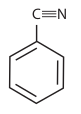
\includegraphics{2021-01-26_17-16_4.png}}
        \subcaptionbox{}{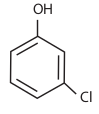
\includegraphics{2021-01-26_17-17.png}}
        \subcaptionbox{}{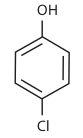
\includegraphics{2021-01-26_17-17_1.png}}
        \subcaptionbox{}{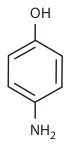
\includegraphics{2021-01-26_17-17_2.png}}
    \end{figure}
\item 如果白光通过溶液后,溶液是蓝色,溶液吸收什么颜色?
\item Beer定律必须满足什么条件?填充下表空白处$T$和$A$的值
    \begin{center}
        \begin{tabular}{lcp{2cm}p{2cm}c}
            \hline
            溶液编号 & 吸收(\%) & \qquad$T$ & $A$ & 浓度(ppm)\\
            \hline
            1  &  1 & & & 1 \\
            2  &  13& & & 6 \\
            3  &  30& & & 15\\
            4  &  55& & & 34\\
            5  &  80& & & 69\\
            \hline
        \end{tabular}
    \end{center}
        
\item 假设上题中获得数据用于标准曲线,并所有测量使用同一样品池,完成下表
    \begin{center}
        \begin{tabular}{lcp{2cm}p{2cm}}
            \hline
            溶液 & 吸收(\%) & \qquad$T$ & 浓度(ppm)\\
            \hline
            A & 30 & & \\
            B & 3 & & \\
            C & 10 & & \\
            D & 50 & & \\
            E & 70 & & \\
            \hline
        \end{tabular}
    \end{center}
\item 样品池长度与吸光度有什么关系?填充下表空白处(浓度相同)
    \begin{center}
        \begin{tabular}{lcc}
            \hline
            样品编号 & 光程$l$ (cm) & A \\
            \hline
            1 & 0.1  & 0.01 \\
            2 & 0.5  & \\
            3 & 1.0  & \\
            4 & 2.0  & \\
            5 & 5.0  & \\
            \hline
        \end{tabular}
    \end{center}
\item 列举三种用于UV/VIS光谱定量分析的试剂,及其用于测定的元素
\item 列举两种荧光试剂。能产生荧光的分子有什么结构特征?
\item 下图是萘和蒽的吸收光谱,结构见谱图。这些分子是将苯环融汇一起的多环芳烃。
    (a)列出这两个分子最大吸收波长和苯的光谱(图\ref{fig:5.12})列表,观察到什么
    趋势?(b)哪些转变导致这些化合物中观察到的峰?(c)解释在最大吸收观察的趋势。
    (d)该系列下一个大分子如下图所示
    \begin{center}
        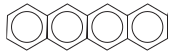
\includegraphics[width=0.35\textwidth]{2021-01-26_16-18.png}
    \end{center}
    预测此并四苯结构最大吸收峰位置,并解释理由。
\item 如图是氧化钬玻璃的UV/VIS吸收光谱,是一种高纯度稀土氧化物玻璃。(a)此光谱与
    有机分子光谱,如图\ref{fig:5.1},吡啶,有什么不同?为什么出现这些不同?(b)
    可以使用该种玻璃做样品池做UV/VIS测试?为什么?
    \begin{center}
        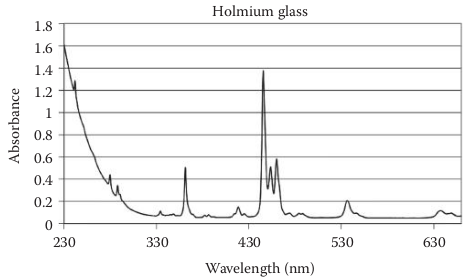
\includegraphics[width=0.75\textwidth]{2021-01-26_16-02.png}
    \end{center}
\end{problemset}
